\documentclass{article}
\usepackage[utf8]{inputenc}
\usepackage{hyperref}
\usepackage{graphicx}
\usepackage{listings}
\usepackage{amssymb}
\usepackage{color}
\usepackage{xcolor}
\usepackage{indentfirst}
\usepackage{makeidx}

\begin{document}
\date{\today}
\title{Jvarkit : java utilities for bioinformatics}
\author{Pierre Lindenbaum PHD\\\href{http://twitter.com/yokofakun}{@yokofakun}\\Institut du Thorax. U1097. Nantes. France.}

\maketitle

\begin{abstract}
Jvarkit ( \url{https://github.com/lindenb/jvarkit} ) is a set of java-based tools for bioinformatics.
\end{abstract}

I don't have written any article about jvarkit yet. This article is a placeholder to get a reference for
Jvarkit ( \url{https://github.com/lindenb/jvarkit} ), a set of more than 100 java-based tools for bioinformatics I've written during the
last years. Most tools have been developped for NGS, for \url{http://biostars.org} \cite{biostar}. Some tools are just 'one-shot'. Some tools like \textbf{SortVCFOnRef} have been deprecated in favor of tools like \textbf{picard/SortVcf} \cite{sortvcf}.


\section{A few tools}

\subsection{VCFFilterJS}
filters a VCF file using a javascript expression.

\subsection{SamJS}
filters a SAM file using a javascript expression.

\subsection{SAM2Tsv}
display a tabular view of each base of the reads vs the reference.

\subsection{Bam2SVG}
display a BAM as SVG (fig.~\ref{fig:Bam2SVG}).

\begin{figure}[!]
 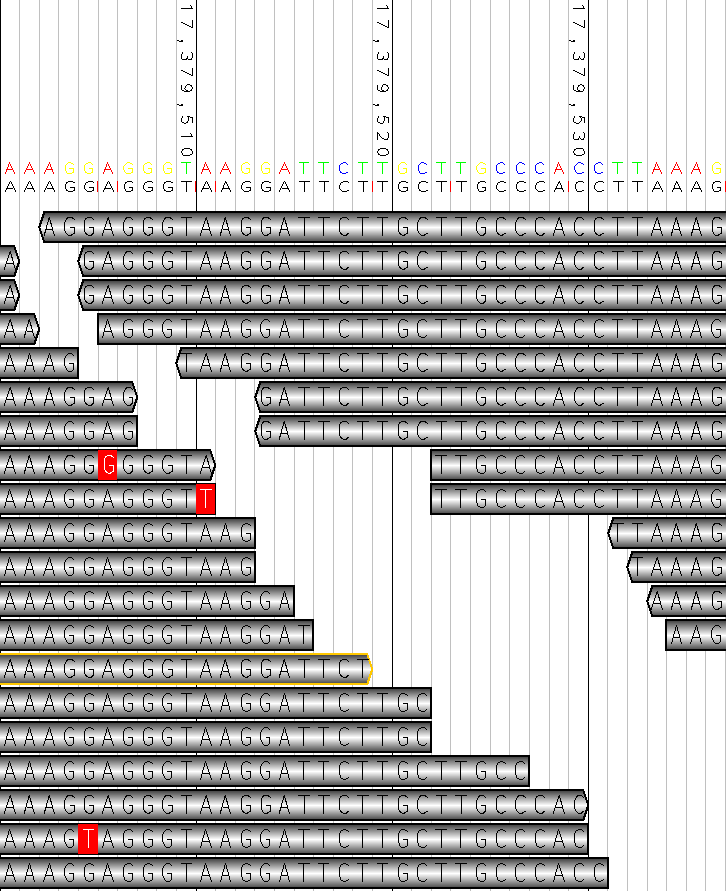
\includegraphics[width=0.8\textwidth]{bam2graphics.png}
 \caption{Bam2SVG}
 \label{fig:Bam2SVG}
\end{figure}

\subsection{Biostar77288}
Low resolution sequence alignment visualization \url{http://www.biostars.org/p/77288/}  (fig.~\ref{fig:Biostar77288}).

\begin{figure}[!]
 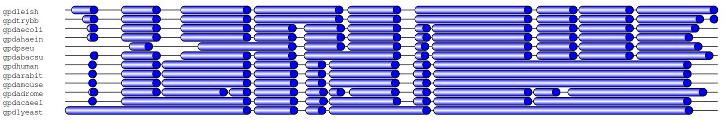
\includegraphics[width=0.8\textwidth]{biostar77288.png}
 \caption{Biostar77288}
 \label{fig:Biostar77288}
\end{figure}

\subsection{SAM4WebLogo}
"Sequence logo ( http://weblogo.berkeley.edu/logo.cgi ) for different alleles or generated from SAM/BAM" http://www.biostars.org/p/73021  (fig.~\ref{fig:SAM4WebLogo}).

\begin{figure}[!]
 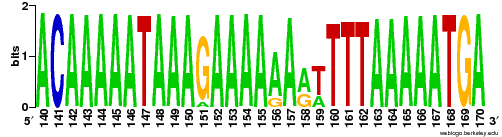
\includegraphics[width=0.8\textwidth]{sam2weblogo.png}
 \caption{SAM4WebLogo}
 \label{fig:SAM4WebLogo}
\end{figure}

\subsection{SigFrame}
SigFrame displays CGH/ position+values in a GUI (fig.~\ref{fig:SigFrame}).

\begin{figure}[!]
 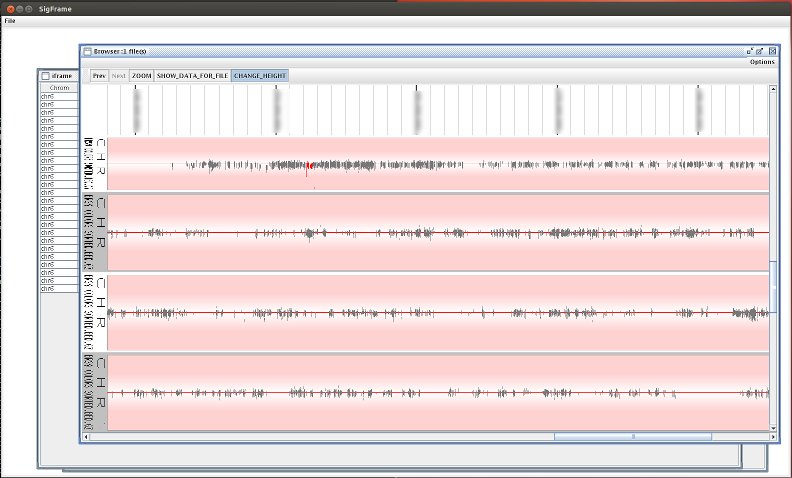
\includegraphics[width=0.8\textwidth]{sigframe.jpg}
 \caption{SigFrame}
 \label{fig:SigFrame}
\end{figure}


\subsection{etc...}
....


\section{Article(s) citing jvarkit}
Articles found using google scholar: 
\begin{itemize}
\item Illumina TruSeq Synthetic Long-Reads Empower De Novo Assembly and Resolve Complex, Highly-Repetitive Transposable Elements.\cite{ext1}
\end{itemize}

\begin{thebibliography}{9}
\bibitem{biostar}
Parnell LD, Lindenbaum P, Shameer K, Dall'Olio GM, Swan DC, Jensen LJ, Cockell SJ, Pedersen BS, Mangan ME, Miller CA, Albert I.
\emph{BioStar: an online question and answer resource for the bioinformatics community.} PLoS Comput Biol. 2011
Oct;7(10):e1002216. doi: 10.1371/journal.pcbi.1002216. Epub 2011 Oct 27. PubMed
PMID: 22046109; PubMed Central PMCID: PMC3203049.

\bibitem{ext1}
Illumina TruSeq Synthetic Long-Reads Empower De Novo Assembly and Resolve Complex, Highly-Repetitive Transposable Elements.
McCoy RC, Taylor RW, Blauwkamp TA, Kelley JL, Kertesz M, et al. (2014) Illumina TruSeq Synthetic Long-Reads Empower De Novo Assembly and Resolve Complex, Highly-Repetitive Transposable Elements. PLoS ONE 9(9): e106689. doi: 10.1371/journal.pone.0106689 

\bibitem{sortvcf}
\url{http://broadinstitute.github.io/picard/command-line-overview.html#SortVcf}

\end{thebibliography}

\end{document}

